\documentclass[14pt, a4paper]{article}
\usepackage[T2A]{fontenc}
\usepackage[utf8]{inputenc}
\usepackage[russian]{babel}
\usepackage[left=3cm, right=1.5cm, top=2cm, bottom=2cm]{geometry}
\usepackage{indentfirst}
\usepackage{microtype}
\usepackage{array}
\usepackage{xcolor}
% \usepackage{times}
\usepackage{tempora}
\usepackage{ulem}
\usepackage{setspace}
\usepackage{amsmath}
\usepackage{booktabs}
\usepackage{graphicx}
\usepackage{float}
\usepackage{listings}
\graphicspath{{reports/figures/}{figures/}}
\lstset{basicstyle=\ttfamily\small, breaklines=true, columns=fullflexible, frame=single, keepspaces=true}
\pagestyle{empty}

\makeatletter
\renewcommand\section{\@startsection {section}{1}{\parindent}%
  {-3.5ex \@plus -1ex \@minus -.2ex}%
  {0.5ex}%
  {\normalfont\Large\bfseries}}
\renewcommand\tableofcontents{%
  \begin{center}\Large\bfseries\contentsname\end{center}%
  \@starttoc{toc}%
}
\renewcommand*\l@section{\@dottedtocline{1}{0em}{1.5em}}
\makeatother

\begin{document}
\onehalfspacing

\begin{center}
    \textbf{ФЕДЕРАЛЬНОЕ ГОСУДАРСТВЕННОЕ АВТОНОМНОЕ ОБРАЗОВАТЕЛЬНОЕ} \\
    \textbf{УЧРЕЖДЕНИЕ ВЫСШЕГО ОБРАЗОВАНИЯ} \\
    \textbf{«МОСКОВСКИЙ АВИАЦИОННЫЙ ИНСТИТУТ} \\
    \textbf{(НАЦИОНАЛЬНЫЙ ИССЛЕДОВАТЕЛЬСКИЙ УНИВЕРСИТЕТ)»}
\end{center}

\begin{center}
    \bfseries Институт №8 «Компьютерные науки и \\
    \bfseries прикладная математика» \\
    \bfseries Кафедра 806 «Вычислительная математика \\
    \bfseries и программирование»
\end{center}

\vspace{3cm}

\begin{center}
    \Large\bfseries Отчет \\
    \vspace{0.5cm}
    \mdseries по лабораторной работе №4.2
\end{center}

\vfill

\noindent
\hfill
\begin{tabular}{ll}
Группа:       & М8О-307Б-21 \\
Студент:      & М. С. Ивченко \\
Преподаватель:& доц. В. В. Киндинова \\
Оценка:       & \underline{\makebox[3cm][c]{}} \\ [0.2cm]
Дата:         & \underline{\makebox[3cm][c]{}}
\end{tabular}

\vfill

\begin{center}
    Москва \\
    2026
\end{center}

\newpage

\setcounter{tocdepth}{2}
\tableofcontents
\newpage

\section*{Тема}
\addcontentsline{toc}{section}{Тема}
Цель данной лабораторной работы -- изучить численные подходы к решению краевых задач для обыкновенных дифференциальных уравнений. В работе сопоставляются метод стрельбы, превращающий краевую задачу в серию задач Коши, и конечно-разностный метод, сводящий задачу к системе алгебраических уравнений.

\section*{Задание}
\addcontentsline{toc}{section}{Задание}
Реализовать метод стрельбы и конечно-разностный метод решения краевой задачи для ОДУ в виде программ. С использованием разработанного программного обеспечения решить краевую задачу для обыкновенного дифференциального уравнения 2-го порядка на указанном отрезке. Оценить погрешность численного решения с использованием метода Рунге-Ромберга и путем сравнения с точным решением.

\section*{Теория}
\addcontentsline{toc}{section}{Теория}
Краевая задача для ОДУ отличается от задачи Коши тем, что условия задаются на разных концах отрезка. Для уравнения второго порядка обычно известны два граничных условия, например линейные комбинации $y(a),y'(a)$ и $y(b),y'(b)$. Требуется найти решение, удовлетворяющее уравнению на всем отрезке и обоим граничным условиям.

Метод стрельбы заменяет краевую задачу задачей Коши с неизвестным начальным параметром $\eta$. Например, если известно $y(a)$, но неизвестно $y'(a)$, то полагают $y'(a)=\eta$ и интегрируют задачу Коши до точки $b$. После этого параметр подбирается так, чтобы правое граничное условие обращалось в ноль:
\[
    \Phi(\eta)=\alpha y(b,\eta)+\beta y'(b,\eta)-\gamma=0.
\]
Таким образом, задача сводится к решению одного нелинейного уравнения относительно $\eta$. Для подбора параметра можно применять метод секущих или Ньютона. Каждый новый параметр требует полного интегрирования задачи Коши, поэтому стоимость метода зависит от числа пробных выстрелов.

В конечно-разностном методе решение ищется сразу в узлах сетки $x_i=a+ih$. Производные заменяются разностными отношениями:
\[
    y'(x_i)\approx\frac{y_{i+1}-y_{i-1}}{2h},\qquad
    y''(x_i)\approx\frac{y_{i-1}-2y_i+y_{i+1}}{h^2}.
\]
После подстановки в дифференциальное уравнение для каждого внутреннего узла получается линейное уравнение относительно $y_{i-1},y_i,y_{i+1}$. Граничные условия задают первое и последнее уравнение системы. В результате краевая задача сводится к трехдиагональной СЛАУ, которую можно решать методом прогонки.

Метод стрельбы хорошо использует уже реализованные методы решения задач Коши, но может быть чувствителен к начальному параметру. Конечно-разностный метод строит глобальную систему сразу и обычно более устойчив для линейных краевых задач. Точность обоих подходов оценивается сравнением с точным решением и методом Рунге--Ромберга при уменьшении шага сетки.

\begin{lstlisting}[language=Python]
matrix[i, i - 1] = a_i / h**2 - b_i / (2*h)
matrix[i, i] = -2 * a_i / h**2 + c_i
matrix[i, i + 1] = a_i / h**2 + b_i / (2*h)
rhs[i] = f_i
\end{lstlisting}

\section*{Ход лабораторной работы}
\addcontentsline{toc}{section}{Ход лабораторной работы}
Решалась краевая задача
\[
    x(x-1)y''-xy'+y=0,\qquad x\in[1,2],
\]
\[
    y'(1)=2,\qquad 2y'(2)-y(2)=1.
\]
Точное решение: $y(x)=1+x+x\ln x$.

Так как при $x=1$ коэффициент при $y''$ равен нулю, в методе стрельбы интегрирование выполнялось справа налево, а параметром было $\eta=y(2)$. Найдено $\eta=4.3834621803$, $\Phi(\eta)=4.44\cdot10^{-16}$.

\begin{figure}[H]
    \centering
    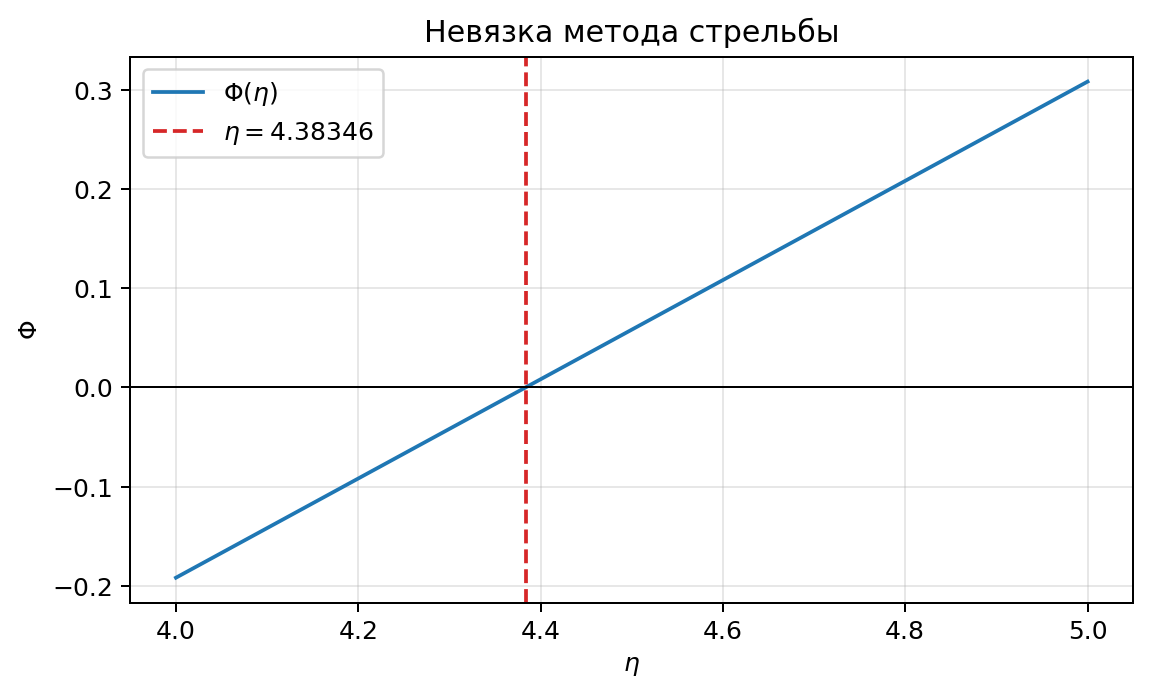
\includegraphics[width=0.86\textwidth]{lab4_2_phi.png}
    \caption{Функция невязки в методе стрельбы.}
\end{figure}

\begin{table}[H]
\centering
\begin{tabular}{lrrr}
\toprule
Метод & $y(1)$ & $y(2)$ & Макс. ошибка на сетке\\
\midrule
Стрельба & 1.9985109838 & 4.3834621803 & 0.0028321808\\
Конечные разности & 2.0000000000 & 4.3865256336 & 0.0004102811\\
Точное решение & 2.0000000000 & 4.3862943611 & 0\\
\bottomrule
\end{tabular}
\caption{Сравнение методов решения краевой задачи.}
\end{table}

\begin{figure}[H]
    \centering
    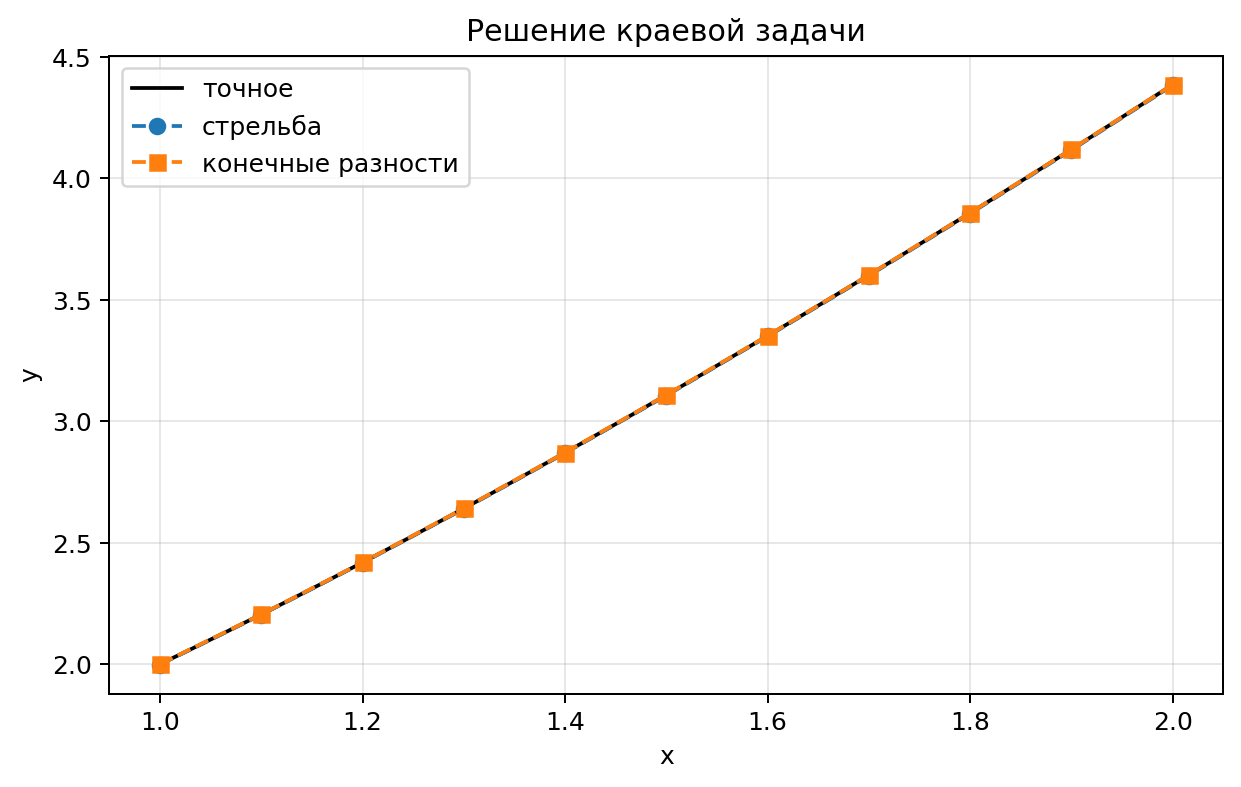
\includegraphics[width=0.86\textwidth]{lab4_2_solutions.png}
    \caption{Решения краевой задачи, найденные двумя методами.}
\end{figure}

\section*{Выводы}
\addcontentsline{toc}{section}{Выводы}
Оба метода дали решение, близкое к точному. Конечно-разностный метод оказался точнее на данной сетке. Для метода стрельбы вырожденность левой границы ухудшает обусловленность после приведения уравнения к виду $y''=f(x,y,y')$, поэтому ошибка около $x=1$ заметнее.

\end{document}
